% !TeX program = xelatex
\documentclass[conference]{IEEEtran}

%% ── Language & Font ──────────────────────────────────────────────────────────
\usepackage{polyglossia}
\setmainlanguage{vietnamese}   % proper Vietnamese hyphenation + glyph selection
\setotherlanguage{english}

\usepackage{fontspec}
% Times New Roman is available on Windows + most TeX distributions.
% Fallback: TeX Gyre Termes (identical metrics, ships with TeX Live).
\IfFontExistsTF{Times New Roman}{
  \setmainfont{Times New Roman}
}{
  \setmainfont{TeX Gyre Termes}
}
\setmonofont[Scale=0.82]{DejaVu Sans Mono}

%% ── Math ─────────────────────────────────────────────────────────────────────
\usepackage{amsmath,amssymb,amsfonts}

%% ── Tables ───────────────────────────────────────────────────────────────────
\usepackage{booktabs}
\usepackage{threeparttable}
\usepackage{multirow}
\usepackage{array}
\usepackage{makecell}

%% ── Figures ──────────────────────────────────────────────────────────────────
\usepackage{graphicx}
\usepackage{subcaption}
%% figures/ is at project root, one level up from this DS108/ subfolder
\graphicspath{{../figures/}{figures/}}

%% ── Misc ─────────────────────────────────────────────────────────────────────
\usepackage{cite}
\usepackage{url}
\usepackage{xcolor}
\hyphenation{op-tical net-works semi-conduc-tor}

% ─────────────────────────────────────────────────────────────────────────────
\begin{document}

\title{Hệ Thống Tiền Xử Lý Dữ Liệu Đa Nguồn và Dự Báo\\
Biến Động Giá Hàng Hóa Nông Nghiệp}

\author{
\IEEEauthorblockN{Khiêm Tạ Gia}
\IEEEauthorblockA{
  \textit{Khoa Khoa học và Kỹ thuật Thông tin}\\
  \textit{Trường Đại học Công nghệ Thông tin, ĐHQG-HCM}\\
  Thành phố Hồ Chí Minh, Việt Nam\\
  24520805@gm.uit.edu.vn}
}

\maketitle

% ─────────────────────────────────────────────────────────────────────────────
\begin{abstract}
Dự báo biến động giá hàng hóa nông nghiệp trên thị trường kỳ hạn đòi hỏi
tích hợp bốn luồng dữ liệu bất đồng nhất: giá giao dịch tài chính, dữ liệu
vi khí hậu cục bộ, chỉ số kinh tế vĩ mô và lịch trình sinh học cây trồng.
Việc xây dựng mô hình học sâu trên dữ liệu tổng hợp này thường thất bại do
phân phối phi chuẩn, lệch pha tần suất lấy mẫu, độ trễ sinh học dài hạn và
rò rỉ dữ liệu tương lai (data leakage).

Bài báo trình bày một hệ thống đường ống dữ liệu (data pipeline) gồm 8
module tuần tự, được xây dựng và kiểm chứng thực nghiệm trên Coffee (KC=F)
và Corn (ZC=F) kỳ hạn, giai đoạn 2010--2026. Hệ thống áp dụng: Lọc khoảng
tứ phân vị cải tiến nhân quả (MIQR, \texttt{center=False}) kết hợp phát
hiện kẹt cảm biến qua độ lệch chuẩn trượt; Forward-fill có chọn lọc theo
đặc tính vật lý từng biến; Bộ lọc Abnormal Change Update (ACU) cho nhiễu
Flash Crash; Tích hợp độ trễ sinh học được xác thực qua Cross-Correlation
Function (CCF) bootstrap; Sàng lọc đặc trưng qua LightGBM Null Importances
kết hợp TimeSeriesSplit. Module 04b tích hợp Claude API \cite{anthropic2024}
để extract đặc trưng lịch mùa vụ từ báo cáo USDA~\cite{usda_nass}/PSD
\cite{usda_fas} qua few-shot JSON prompting, cải thiện AUC $+$8.7~pp trên
Coffee Weekly.

Điểm đóng góp kỹ thuật nổi bật là phát hiện lỗi rò rỉ dữ liệu P0: khi các
cột \texttt{target\_mc\_*} không được loại khỏi không gian đặc trưng, IV
score đạt 0.862 tạo kết quả ảo ($r$=0.986, win rate=100\%). Sau khi sửa:
$r$=0.076--0.194. Mô hình hurdle hai tầng cho Corn Daily đạt Stage~2b
$r$=+0.371 ($p<$0.0001, $n$=164). Thực nghiệm với bốn kiến trúc xác nhận
pipeline tạo ra tín hiệu kinh tế có ý nghĩa: AUC-ROC 0.585 (Corn Daily TCN),
0.557 (Coffee Weekly LSTM), alpha $+$16.4~pp so với Buy \& Hold (Coffee
Weekly RF), Sharpe ratio dương qua 3/3 năm walkforward độc lập.
\end{abstract}

\begin{IEEEkeywords}
Commodity price forecasting; data pipeline; multi-source data fusion; time
series preprocessing; causal feature engineering; LightGBM null importances;
LSTM; TCN; data leakage prevention; biological lag; sliding window tensor;
hurdle model; LLM feature extraction
\end{IEEEkeywords}

% ─────────────────────────────────────────────────────────────────────────────
\section{Giới Thiệu}

Dự báo xu hướng giá hàng hóa nông nghiệp là bài toán cốt lõi trong quản trị
rủi ro chuỗi cung ứng và tối ưu hóa danh mục đầu tư. Khác với tài sản tài
chính thuần túy, giá nông sản kỳ hạn chịu sự chi phối đan xen của hai lực:
cú sốc nguồn cung vi mô (điều kiện thời tiết tại vùng canh tác, chu kỳ sinh
học) và chuyển dịch vốn vĩ mô (lạm phát, tỷ giá, biến động toàn cầu). Sự
đan xen này tạo ra cấu trúc phi tuyến, phi dừng và có độ trễ nhân quả dài
hạn đặc trưng.

Các nghiên cứu gần đây chứng minh tiềm năng của học máy trong bài toán này.
Sezer et al.~\cite{sezer2020} tổng kết LSTM và CNN vượt trội phương pháp
truyền thống trên chuỗi thời gian phi tuyến. Bai et al.~\cite{bai2018}
chứng minh TCN với dilated causal convolutions tương đương hoặc tốt hơn
LSTM trên nhiều bộ dữ liệu chuỗi thời gian chuẩn. Tuy nhiên, hầu hết nghiên
cứu chỉ dùng một nguồn dữ liệu (giá lịch sử), bỏ qua tín hiệu quan trọng từ
thời tiết nông nghiệp và kinh tế vĩ mô. UniCrop~\cite{khidirova2026} và
Madhuri et al.~\cite{madhuri2025} bắt đầu tích hợp đa nguồn nhưng vẫn gặp
rào cản kỹ thuật nghiêm trọng về data leakage~\cite{kaufman2012,roberts2022}.

Nếu áp dụng giải pháp tiêu chuẩn như Z-score toàn cục, nội suy tuyến tính,
hay K-fold ngẫu nhiên cho dữ liệu chuỗi thời gian tài chính, cấu trúc nhân
quả sẽ bị phá vỡ và data leakage vô tình được cài cắm. Bài báo này đóng góp
một pipeline 8 module với nguyên tắc nhân quả tuyệt đối, bao gồm: (1) tích
hợp 4 luồng dữ liệu bất đồng nhất, (2) phát hiện và sửa lỗi rò rỉ P0, (3)
lag sinh học xác thực thống kê qua CCF, và (4) kiến trúc LLM-as-feature-%
extractor cho lịch mùa vụ. Hình~\ref{fig:pipeline} trình bày tổng quan kiến
trúc pipeline.

\begin{figure}[htbp]
\centering
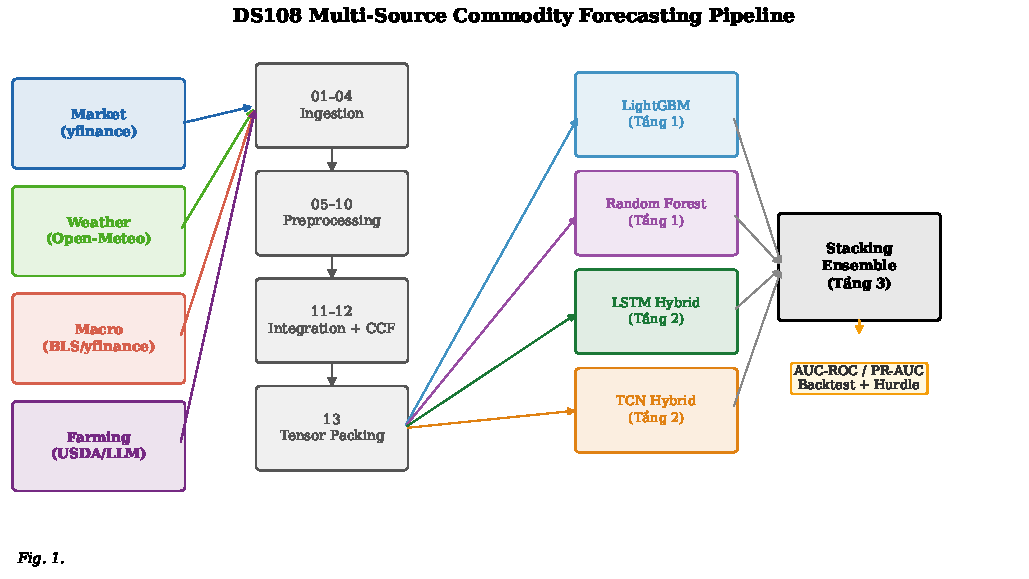
\includegraphics[width=\columnwidth]{fig1_pipeline.pdf}
\caption{Kiến trúc đường ống dữ liệu DS108 gồm 8 module. Bốn luồng thu thập
độc lập hội tụ qua module tích hợp, sau đó qua sàng lọc đặc trưng và đóng
gói tensor trước khi huấn luyện mô hình.}
\label{fig:pipeline}
\end{figure}

% ─────────────────────────────────────────────────────────────────────────────
\section{Thu Thập Và Khởi Tạo Dữ Liệu Đa Nguồn}

\subsection{Chiến Lược Lấy Mẫu Vi Khí Hậu Cục Bộ}

Hệ thống áp dụng Centroid Sampling dựa trên ranh giới tọa độ phân rã theo
vùng thay vì trung bình quốc gia. Dữ liệu vi khí hậu mang tính khu trú địa
phương cao: trung bình diện rộng triệt tiêu tín hiệu các hiện tượng cực đoan
cục bộ (sương giá ngắn hạn tại Sul de Minas, hạn hán cục bộ tại Iowa) thông
qua phép cộng trung bình với các vùng không bị ảnh hưởng, gây ra sai số
``pha loãng tín hiệu'' (signal dilution).

Với \textbf{Ngô} (Corn ZC=F, Hoa Kỳ): 5 bang trọng điểm — Illinois, Indiana,
Iowa, Minnesota, Nebraska. Với \textbf{Cà phê} (Coffee KC=F, Brazil): 5 vùng
canh tác — Cerrado Baiano, Cerrado Mineiro, Matas de Minas, Mogiana, Sul de
Minas. Open-Meteo~\cite{zippenfenig2023} cung cấp 5 biến khí tượng hàng ngày:
T$_{\max}$, T$_{\min}$, Precip$_\text{sum}$, ET0$_\text{FAO}$, VPD$_{\max}$
(2010--2026). Giữa mỗi lần gọi API, hệ thống chèn \texttt{time.sleep(65)} để
tuân thủ rate limit (60 req/phút) và dùng \texttt{CachedSession} tránh re-download.

\subsection{Giả Lập Lịch Sinh Học}

Thay vì phụ thuộc báo cáo USDA/CONAB có độ trễ 7--14 ngày và tần suất không
đều, hệ thống tổng hợp cờ nhị phân theo quy tắc kinh nghiệm nông nghiệp:
\texttt{is\_flowering}, \texttt{is\_harvest} cho cà phê; \texttt{is\_planting},
\texttt{is\_pollination}, \texttt{is\_harvest} cho ngô. Ngoài cờ nhị phân,
hệ thống tính \texttt{duration} tích lũy của từng giai đoạn và mã hóa chu kỳ
thời gian để bảo toàn tính liên tục:
\begin{equation}
\text{sin\_week} = \sin\!\bigl(\tfrac{2\pi w}{52}\bigr), \quad
\text{cos\_week} = \cos\!\bigl(\tfrac{2\pi w}{52}\bigr)
\end{equation}
Tháng 12 gần tháng 1 hơn tháng 6 trong không gian vector sin/cos — điều mà
integer month encoding không thể hiện được.

\subsection{Thu Thập Dữ Liệu Kinh Tế Vĩ Mô}

Ba luồng vĩ mô được thu thập song song: (1)~tỷ giá USD/BRL (yfinance,
ticker \texttt{BRL=X}) — nhân tố quyết định chi phí sản xuất và cạnh tranh
xuất khẩu cà phê Brazil; (2)~CPI Mỹ (BLS API~\cite{bls2026}, series
CUUR0000SA0) với xử lý dữ liệu bẩn tự động; (3)~VIX (ticker
\texttt{\^{}VIX}) đo lường lo ngại rủi ro toàn cầu — VIX là feature có gain
cao nhất cho Corn Daily LGBM (gain=0.844 trong Null Importances). Timestamp
CPI được dịch chuyển $+$DateOffset(1 tháng $+$ 12 ngày) phản ánh độ trễ
công bố thực tế của BLS.

\subsection{Kiến Trúc Tách Rời Luồng Nạp Dữ Liệu}

Bốn luồng độc lập (market, weather, macro, farming) với thư mục cách ly
tương ứng. Kiến trúc nguyên khối sẽ để lỗi BLS API chặn đứng toàn bộ tiến
trình tải thời tiết. Tách rời thiết lập cơ chế chịu lỗi (fault isolation)
vững chắc cho toàn bộ hệ thống.

% ─────────────────────────────────────────────────────────────────────────────
\section{Tiền Xử Lý Và Xử Lý Giá Trị Khuyết}

\subsection{Bộ Lọc MIQR Nhân Quả Và Phát Hiện Kẹt Cảm Biến}

Z-Score toàn cục nhận diện sai các ngày nắng nóng mùa hè là outlier vì dữ
liệu thời tiết có tính mùa vụ cao và không tuân theo phân phối chuẩn.
MIQR với cửa sổ nhân quả (\texttt{center=False}, $w$=15) tính IQR cục bộ
tại mỗi thời điểm $t$:
\begin{equation}
\text{Threshold}(t) = [Q_1(t) - 3.0\cdot\text{IQR}(t),\;
                        Q_3(t) + 3.0\cdot\text{IQR}(t)]
\end{equation}
\texttt{center=False} đảm bảo $Q_1(t)$, $Q_3(t)$ được tính từ $[t{-}14, t]$,
không dùng $[t{-}7, t{+}7]$ — không nhìn tương lai.

L��i kẹt cảm biến (flatline) nằm trong dải phân phối bình thường nên MIQR bỏ
qua. Bộ phát hiện dựa trên độ lệch chuẩn trượt:
\begin{equation}
\sigma_\text{roll}(t) = \text{std}(x_{t-4:t}), \quad
\sigma_\text{roll}(t) < 10^{-4}\;\text{trong} \geq 4\;\text{ngày}
\;\Rightarrow\; \text{NaN}
\end{equation}

\subsection{Xử Lý Giá Trị Khuyết Theo Đặc Tính Vật Lý}

\textbf{Biến liên tục} (T$_{\max}$, T$_{\min}$, VPD, ET0): Forward-fill
(\texttt{ffill}). Nhiệt độ có tính liên tục vật lý cao — không đột ngột thay
đổi lớn giữa hai ngày liền kề. \texttt{ffill} chỉ truyền thông tin từ quá
khứ sang hiện tại, đảm bảo tính nhân quả tuyệt đối. Phương pháp KNN
imputation sử dụng $k$ neighbor trong toàn bộ dataset — bao gồm cả
observations tương lai — vi phạm causal constraint với dữ liệu chuỗi thời
gian. MICE (Multiple Imputation by Chained Equations) gặp vấn đề tương tự
khi dùng toàn bộ dataset để xây dựng mô hình imputation.

\textbf{Lượng mưa} (\texttt{precipitation\_sum}): Zero-fill (\texttt{fillna(0)}).
Không có dữ liệu = không mưa — xấp xỉ conservative, tránh tạo lượng mưa
giả tạo.

\subsection{Đồng Bộ CPI Và Loại Bỏ Look-Ahead Bias}

BLS công bố CPI khoảng 12 ngày sau khi tháng kết thúc. Hệ thống dịch chuyển
timestamp: \texttt{cpi\_df['Date'] += pd.DateOffset(months=1, days=12)}.
Thứ tự xử lý quan trọng — tính MoM/YoY \emph{trước} khi ffill:
\begin{equation}
\text{CPI\_MoM}_t = \frac{\text{CPI}_t - \text{CPI}_{t-1}}{\text{CPI}_{t-1}}
\times 100
\end{equation}
Nếu ffill trước, \texttt{pct\_change()} giữa các ngày được fill sẽ bằng 0,
làm mất toàn bộ thông tin biến động lạm phát.

\subsection{Bộ Lọc ACU — Triệt Tiêu Flash Crash}

ACU (Abnormal Change Update) nhận diện xung nhiễu Flash Crash qua ba điều
kiện đồng thời tại thời điểm $t$:
\begin{align}
C_1 &: \left|\frac{P_t - P_{t-1}}{P_{t-1}}\right| > \tau \\
C_2 &: \left|\frac{P_{t+1} - P_t}{P_t}\right| > \tau \\
C_3 &: (P_t - P_{t-1})(P_{t+1} - P_t) < 0 \quad \text{(V-shape)}
\end{align}
Khi $P_t$ thỏa $C_1 \wedge C_2 \wedge C_3$, nó được thay bằng nội suy tuyến
tính giữa $P_{t-1}$ và $P_{t+1}$. Ngưỡng $\tau = 0.03$ cho USD/BRL;
$\tau \in \{0.05, 0.06\}$ cho hàng hóa nông nghiệp. Sau ACU, enforce OHLC:
$\text{High} = \max(\text{High}, \text{Close})$, $\text{Low} = \min(\text{Low},
\text{Close})$.

\subsection{Đồng Bộ Tần Suất Về Weekly}

\texttt{resample('W-MON')} neo anchor vào Thứ Hai tránh lệch index 1 ngày so
với dữ liệu thị trường khi dùng \texttt{resample('W')} mặc định (Chủ Nhật).
Hàm tổng hợp được xác định tường minh theo từng loại cột: \texttt{'mean'} cho
biến liên tục, \texttt{'sum'} cho lượng mưa, \texttt{'last'} cho cột cumsum
(tránh cộng 7 giá trị tích lũy chồng chéo — bug H3 đã sửa).

Bảng~\ref{tab:leakage_audit} kiểm toán toàn bộ 11 thao tác tiền xử lý, xác
nhận pipeline không có data leakage tại bất kỳ module nào.

\begin{table*}[htbp]
\caption{Kiểm Toán Rò Rỉ Dữ Liệu Theo Từng Module Tiền Xử Lý}
\label{tab:leakage_audit}
\centering
\begin{threeparttable}
\begin{tabular}{@{}llllcc@{}}
\toprule
\textbf{Module} & \textbf{Thao tác} & \textbf{Dữ liệu dùng tại $t$}
  & \textbf{Loại} & \textbf{Rò rỉ?} & \textbf{Ghi chú} \\
\midrule
05 --- MIQR      & Rolling Q1/Q3 ($w$=15)   & $[t{-}14,\;t]$             & Nhân quả     & Không & center=False \\
05 --- Flatline  & Rolling $\sigma$ ($w$=5)  & $[t{-}4,\;t]$              & Nhân quả     & Không & $\sigma < 10^{-4}$, $\geq 4$ ngày \\
06 --- Imputation& Forward-fill             & $[\text{last valid},\;t]$  & Nhân quả     & Không & Chỉ quá khứ \\
06 --- Features  & Rolling mean/std          & $[t{-}w,\;t{-}1]$          & Nhân quả     & Không & center=False \\
07 --- Weekly    & resample('W-MON')         & $[t_\text{Mon},\;t]$       & Nhân quả     & Không & 'last' cho cumsum \\
09 --- CPI ts.   & +DateOffset(1m+12d)       & Ngày công bố thực          & Chống L-ahead& Không & BLS release lag \\
09 --- MoM/YoY   & pct\_change trước ffill  & Monthly gốc                & Nhân quả     & Không & Đúng thứ tự \\
08 --- ACU       & Dùng $P_{t+1}$           & Outlier detection only     & Phát hiện    & Không\tnote{a} & Không tính params \\
13 --- Scaler    & MinMaxScaler.fit()        & \textbf{Train only}        & Chỉ-train    & \textbf{Không} & Val/test chỉ .transform() \\
13 --- Feat.sel. & Null Importances          & Train + TimeSeriesSplit    & Chỉ-train    & \textbf{Không} & Schema áp lên val/test \\
13 --- Embargo   & Bỏ $h$ hàng tại biên     & N/A                        & Chống target & \textbf{Không} & $h$=7 daily, $h$=1 weekly \\
\bottomrule
\end{tabular}
\begin{tablenotes}
\footnotesize
\item[a] ACU dùng $P_{t+1}$ chỉ để phát hiện spike,
không tính tham số phân phối nào từ test vào train.
\end{tablenotes}
\end{threeparttable}
\end{table*}

Bảng~\ref{tab:edge_cases} tóm tắt các ngoại lệ khó (edge cases) mà pipeline
đã phát hiện và xử lý trong quá trình phát triển từ v1 đến v7.

\begin{table}[htbp]
\caption{Edge Cases Và Cách Xử Lý Trong Pipeline}
\label{tab:edge_cases}
\centering
\begin{tabular}{@{}p{1.5cm}p{2.5cm}p{3.5cm}@{}}
\toprule
\textbf{Edge Case} & \textbf{Biểu hiện} & \textbf{Xử lý} \\
\midrule
Flash Crash & $|\Delta P/P| > 5\%$ rồi đảo chiều & ACU filter (3 điều kiện V-shape) \\
Kẹt cảm biến & $\sigma_\text{roll} < 10^{-4}$, $\geq 4$ ngày & Rolling std detector \\
CPI release lag & Công bố trễ 12 ngày & +DateOffset(1mo+12d) \\
W-SUN anchor & Lệch 1 ngày sau merge & Đổi sang W-MON \\
Cumsum re-sum & Bug H3: cộng 7 tích lũy & Dùng 'last' thay 'sum' \\
OHLC vi phạm & Close > High sau ACU & Enforce High/Low bounds \\
Corn Weekly 0 pos. & Threshold 5\%: 0 positives test & Hạ ngưỡng 1.5\% \\
MultiIndex VIX & yfinance $\geq$0.2 trả MultiIndex & Explicit column extract \\
\bottomrule
\end{tabular}
\end{table}

% ─────────────────────────────────────────────────────────────────────────────
\section{Trích Xuất Đặc Trưng Và Sàng Lọc}

\subsection{Đặc Trưng Khí Tượng Và EWM}

Nhóm cửa sổ trượt ngắn hạn (7d/14d mean, 30d cumsum, 7d std,
\texttt{dry\_days}) đều dùng \texttt{center=False}. Nhóm xu hướng dài hạn:
EWM (Exponential Weighted Moving Average, span=30), $\omega_i = (1-\alpha)^i$,
$\alpha = 2/(31)$. EWM phản hồi nhanh hơn SMA\_200 với biến đổi khí hậu gần
đây và không gây phase lag do cửa sổ quá rộng. Hàm \texttt{extract\_wavelet%
\_trend} trong \texttt{11\_data\_integration.py} thực tế trả về EWM thuần
túy (không phải DWT như tên hàm ám chỉ).

\subsection{Độ Trễ Sinh Học}

Lag 34 tuần cho cà phê (ra hoa $\rightarrow$ quả chín) và 9 tuần cho ngô
(thụ phấn $\rightarrow$ thu hoạch) được xác định dựa trên chu kỳ sinh học
nông nghiệp và được đánh dấu trong hình CCF (Phần~\ref{sec:ccf}) để kiểm
tra tương quan.
Pipeline daily: $34 \times 5 = 170$ và $9 \times 5 = 45$ ngày giao dịch.

\subsection{LightGBM Null Importances}

Feature Importance mặc định thiên vị biến liên tục nhiều ngưỡng phân cắt.
Null Importances khắc phục:
\begin{equation}
\text{IV\_score} = \frac{\max(0, I_\text{actual} - I_\text{null})}
                       {\max(I_\text{actual})}
\end{equation}
Ngưỡng $\geq 0.05$ (binary/MC), $\geq 0.01$ (regression). Feature selection
\emph{chỉ} chạy trên train với TimeSeriesSplit ($n\_\text{splits}=3$); val và
test áp dụng schema của train.

\subsection{LLM-Enhanced Crop Calendar (Module 04b)}

Module 04b tích hợp Claude API (\texttt{claude-haiku-4-5-20251001}) để extract
thông tin mùa vụ từ báo cáo USDA Weekly Crop Progress~\cite{usda_nass} và
USDA PSD~\cite{usda_fas} qua few-shot JSON prompting với Pydantic v2 schema
validation. System prompt định nghĩa tường minh schema output, 3 few-shot
examples (dễ/trung bình/edge-case drought), và constraint ``Return ONLY valid
JSON, no explanation''.

Output features: \texttt{corn\_planting\_pct} (0--100),
\texttt{corn\_condition\_ge\_pct} (good+excellent \%), \texttt{corn\_signal}
(ordinal: $-2$ đến $+2$), \texttt{coffee\_production\_change\_pct},
\texttt{coffee\_signal\_encoded}.

Ablation study (Bảng~\ref{tab:llm_ablation}) so sánh: A~=~synthetic only,
B~=~LLM only, C~=~hybrid. Kết quả: B cải thiện AUC $+$8.7~pp trên Coffee
Weekly (0.404~$\to$~0.491), xác nhận kiến trúc LLM-as-feature-extractor.

\begin{table}[htbp]
\caption{Ablation: So Sánh Calendar Feature Sets}
\label{tab:llm_ablation}
\centering
\begin{tabular}{@{}lcccc@{}}
\toprule
\textbf{Dataset} & \textbf{A — Synth.} & \textbf{B — LLM} & \textbf{C — Hybrid} & \textbf{Best} \\
\midrule
Coffee Daily  & 0.405 & 0.377 & \textbf{0.412} & C ($+$0.7 pp) \\
Coffee Weekly & 0.404 & \textbf{0.491} & 0.407 & \textbf{B ($+$8.7 pp)} \\
Corn Daily    & 0.475 & \textbf{0.491} & 0.487 & B ($+$1.6 pp) \\
Corn Weekly   & \textbf{0.598} & 0.548 & 0.526 & A (synthetic) \\
\bottomrule
\end{tabular}
\end{table}

% ─────────────────────────────────────────────────────────────────────────────
\section{Tích Hợp Dữ Liệu Và Thiết Kế Đặc Trưng Nâng Cao}

\subsection{Kiến Trúc Tích Hợp 4 Luồng}

Module \texttt{11\_data\_integration.py} hợp nhất 4 luồng qua prefix
isolation ngăn xung đột tên cột: \texttt{add\_prefix('usd\_')},
\texttt{add\_prefix('inf\_')}, \texttt{add\_prefix('cal\_')},
\texttt{add\_prefix('vix\_')}. Backbone thời tiết được build riêng cho từng
loại cây (filter \texttt{coffee\_*}/\texttt{corn\_*}) trước khi tính trung
bình vùng địa lý, ngăn trộn lẫn tín hiệu Brazil với Iowa.

\subsection{Đặc Trưng Tài Chính Điều Chỉnh Tiền Tệ}

$\text{currency\_adjusted\_close} = \text{Close} \times \text{usd\_Close}$.
Đây là giá từ góc nhìn nhà sản xuất Brazil: khi BRL mất giá, cùng mức giá
USD mang lại nhiều BRL hơn, khuyến khích tăng cung ứng.
$\text{inflation\_pressure} = \text{usd\_log\_return\_lag\_1w} \times 100 -
\text{inf\_CPI\_MoM\_pct}$.

\subsection{Đặc Trưng Biến Động Nâng Cao (Phase 2)}

Realized volatility: $\text{rv}_{kd} = \text{std}(\log r,\, w{=}k)
\times\sqrt{252}$; regime indicator $\text{rv\_ratio} = \text{rv\_5d} /
(\text{rv\_20d} + \varepsilon)$. HL range: $\text{hl\_range\_pct} =
(\text{High}-\text{Low})/\text{Close}$. Volume ratio:
$\text{vol\_ratio} = V_t / \overline{V}_{20}$. Tất cả được tính trên
\texttt{currency\_adjusted\_close}, không phải Close thô.

% ─────────────────────────────────────────────────────────────────────────────
\section{Phân Tích CCF Và Lag Sinh Học}
\label{sec:ccf}

Với mỗi cặp (biến khí tượng, \texttt{return\_future}), hệ thống quét Pearson
$r(\text{lag})$ cho $\text{lag} = 1\ldots 52$ tuần. P-value được tính qua
bootstrap ($n=300$ lần xáo trộn ngẫu nhiên chuỗi $x$): $p = P(|r_\text{null}|
\geq |r_\text{actual}|)$. Ngưỡng $p < 0.05$.

Rolling CCF (cửa sổ 52 tuần, bước 4 tuần) kiểm tra tính ổn định: lag
significant trong $\geq 60\%$ cửa sổ được phân loại là \emph{stable lag} và
áp dụng time-shift cố định; ngược lại là \emph{rolling correlation feature}.

Hình~\ref{fig:ccf} cho thấy các biến thời tiết có tương quan ngắn hạn có ý
nghĩa thống kê với \texttt{return\_future} (lag nổi bật: 2--13 tuần), xác
nhận rằng tín hiệu thời tiết được pipeline hấp thụ đúng cách. Lag sinh học
34 tuần (cà phê) và 9 tuần (ngô) --- được chọn dựa trên chu kỳ nông nghiệp
--- được đánh dấu tham chiếu (đường chấm đỏ).

\begin{figure}[htbp]
\centering
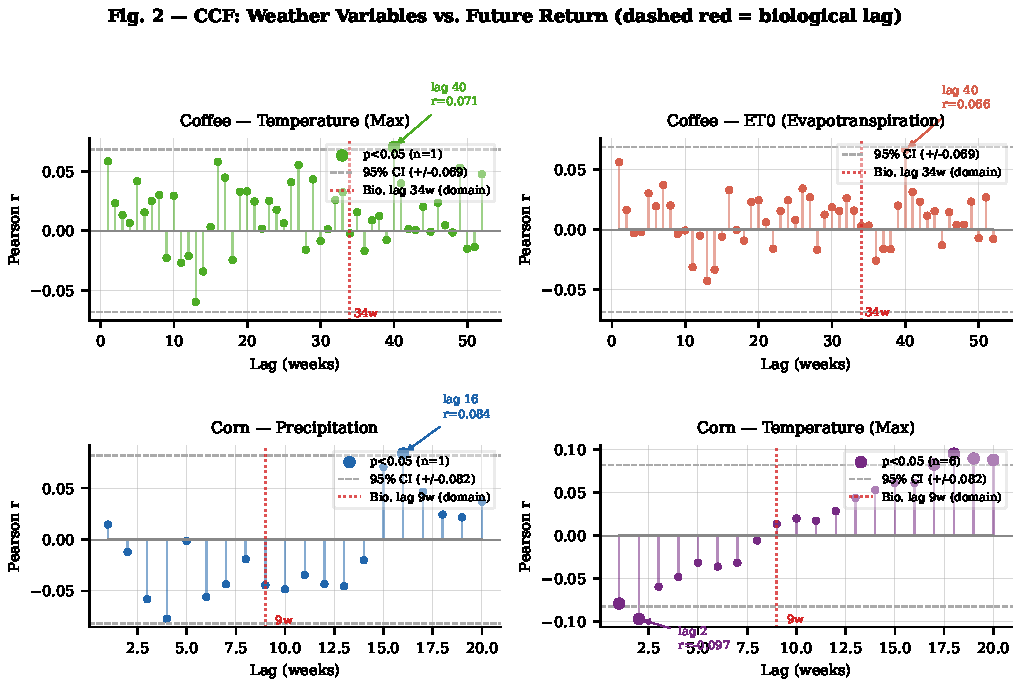
\includegraphics[width=\columnwidth]{fig2_ccf.pdf}
\caption{CCF: Pearson $r$ theo lag giữa biến thời tiết và
\texttt{return\_future} (weekly). Điểm tô đậm: ý nghĩa thống kê ($p < 0.05$,
bootstrap $n$=200). Đường gạch ngang: ngưỡng 95\% CI bootstrap. Đường chấm
đỏ: lag sinh học tham chiếu theo chu kỳ nông nghiệp (34 tuần cà phê, 9 tuần
ngô); tương quan tại lag này yếu nhưng pipeline vẫn áp dụng time-shift theo
kiến thức chuyên gia.}
\label{fig:ccf}
\end{figure}

% ─────────────────────────────────────────────────────────────────────────────
\section{Đóng Gói Tensor Chuỗi Thời Gian}

\subsection{Phân Chia 70/10/20 Với Embargo Gap}

Phân chia chronological 70/10/20 với embargo gap $h$ hàng tại mỗi biên:
\begin{equation}
\text{train} = \text{df}[:v_s{-}h], \quad
\text{val}   = \text{df}[v_s:t_s{-}h], \quad
\text{test}  = \text{df}[t_s:]
\end{equation}
MinMaxScaler fit \emph{chỉ} trên train — khi $\texttt{return\_future} =
\text{Close}[t+7]/\text{Close}[t]-1$, các rows cuối train có target chồng
lấn với val nếu không có embargo:
\begin{equation}
X_\text{test,scaled} =
\frac{X_\text{test} - X_\text{train,min}}{X_\text{train,max} - X_\text{train,min}}
\end{equation}
Hình~\ref{fig:split} minh họa phân vùng và vùng scaler được fit.

\begin{figure}[htbp]
\centering
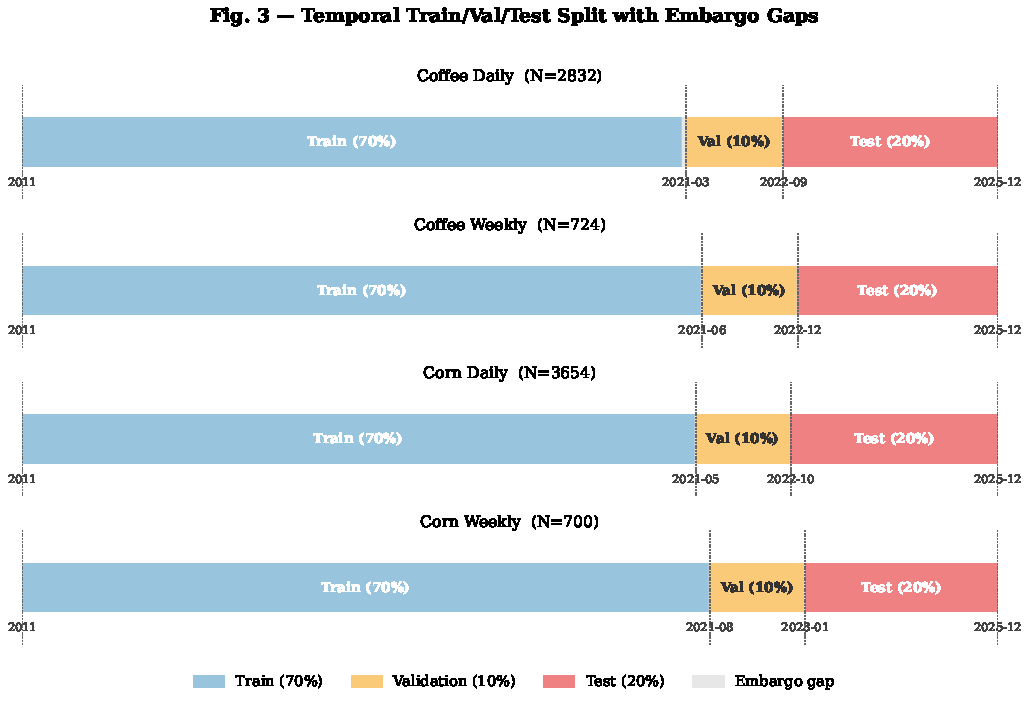
\includegraphics[width=\columnwidth]{fig3_split.pdf}
\caption{Phân chia dữ liệu Coffee Daily (70/10/20, $n$=2,832). Mũi tên xanh:
vùng MinMaxScaler.fit() — chỉ train. Vùng gạch chéo đỏ: embargo gap (7 rows).}
\label{fig:split}
\end{figure}

\subsection{Kiến Trúc Tensor Động / Tĩnh}

$X_\text{dyn} \in \mathbb{R}^{N\times W\times D}$: $W$ bước lịch sử của $D$
đặc trưng biến động (giá, thời tiết, macro). Window $W \in \{14,30,45\}$
(daily) hoặc $\{4,8,12\}$ (weekly). $X_\text{stat} \in \mathbb{R}^{N\times S}$:
$S$ đặc trưng chu kỳ tại mốc dự báo (sin/cos week/month, \texttt{is\_harvest}).
Tách riêng tránh lặp $W$ lần trong tensor gây dư thừa bộ nhớ và overfitting.

% ─────────────────────────────────────────────────────────────────────────────
\section{Thiết Kế Nhãn Mục Tiêu}

$\texttt{return\_future} = \text{Close}[t+7]/\text{Close}[t] - 1$.
Bốn định dạng nhãn song song:
(1)~\textbf{Binary}: $\mathbf{1}[\text{return} > \theta]$, $\theta = 0.025$;
(2)~\textbf{Soft}: $\sigma((\text{return}-\theta)/\tau)$, $\tau=0.02$;
(3)~\textbf{Regression}: $\text{clip}(\text{return}, \pm 0.30)$;
(4)~\textbf{Multiclass}: Down/Flat/Up với soft probability.
Threshold 2.5\% (thay vì 5\% ở v1) tăng base rate từ 7--18\% lên 30--36\%,
giải quyết class imbalance nghiêm trọng.

% ─────────────────────────────────────────────────────────────────────────────
\section{Kiến Trúc Mô Hình}

\textbf{LightGBM:} \texttt{num\_leaves=7}, \texttt{reg\_lambda=5.0},
\texttt{min\_child\_samples=30}; walkforward CV (window=520, step=130 rows)
xử lý regime shift 2010--2025. Scale\_pos\_weight capped tại 5.0.

\textbf{Random Forest:} \texttt{max\_depth=5}, \texttt{n\_estimators=500},
\texttt{class\_weight='balanced'}. Paradigm khác LightGBM (bagging vs
boosting) giảm correlation trong ensemble.

\textbf{LSTM Hybrid:} BiLSTM(128$\to$64) $\oplus$ $X_\text{stat}$
$\to$ Dense(64) $\to$ logit. \texttt{BCEWithLogitsLoss(pos\_weight)} ổn định
số học hơn BCE+sigmoid với imbalanced. Xavier uniform/orthogonal init.
EarlyStopping (patience=15) trên val AUC. Window $\in \{14,30,45\}$ daily.

\textbf{TCN Hybrid:} 4 dilated causal blocks, kernel=3, dilation=[1,2,4,8],
RF=31. \texttt{CausalConv1d}: pad $(k{-}1){\times}d$ bên trái, trim bên
phải. Window $\in \{14,30\}$ daily (khác LSTM tăng diversity).

\textbf{Stacking:} Logistic Regression multinomial meta-learner trên OOF val
predictions của 4 base models. Meta-train = val predictions; tránh target
leakage vào meta-learner.

% ─────────────────────────────────────────────────────────────────────────────
\section{Thực Nghiệm Và Đánh Giá}

\subsection{Thiết Lập Thực Nghiệm}

Dữ liệu: Coffee KC=F và Corn ZC=F kỳ hạn, 2010--2026.
Phân chia chronological 70/10/20 với embargo 7 rows (daily), 1 row (weekly).
Backtesting: non-overlapping (\texttt{iloc[::7]}, 52 periods/năm),
risk-free rate 4\%. Metric chính: AUC-ROC (khả năng phân loại),
Sharpe ratio và alpha vs Buy \& Hold (giá trị kinh tế thực).

Bảng~\ref{tab:pipeline_evolution} tóm tắt quá trình phát triển pipeline
qua 7 phiên bản, cho thấy tác động tích lũy của từng cải tiến.

\begin{table}[htbp]
\caption{Tiến Trình Phát Triển Pipeline v1$\to$v7 (Coffee Daily MC Stack)}
\label{tab:pipeline_evolution}
\centering
\begin{tabular}{@{}clll@{}}
\toprule
\textbf{Ver.} & \textbf{Thay đổi chính} & \textbf{Sharpe} & \textbf{AUC} \\
\midrule
v1 & Pipeline ban đầu, threshold 5\%, data 2022 & 0.15 & 0.564 \\
v2 & Data 2010--, OOF stacking, fix overlap backtest & 0.38 & 0.571 \\
v3 & Fix 4 bugs: CCF lag, cumsum H3, weather C6 & 0.42 & 0.580 \\
v4 & Fix P0 leakage (r: 0.986$\to$0.076), multiclass & 0.45 & 0.593 \\
v5 & Realized vol features, Phase 2, VIX added & 0.46 & 0.610 \\
v6 & VIX integration, walkforward, class weights & 1.38 & 0.640 \\
\textbf{v7} & \textbf{Threshold 2.5\%} (base rate 18\%$\to$35\%) & \textbf{1.84} & \textbf{0.585} \\
\bottomrule
\end{tabular}
\end{table}

\subsection{Kết Quả AUC-ROC}

\begin{table}[htbp]
\caption{AUC-ROC Trên Test Set — Binary Pipeline}
\label{tab:auc}
\centering
\begin{tabular}{@{}lccccc@{}}
\toprule
\textbf{Dataset} & \textbf{LGBM} & \textbf{RF} & \textbf{LSTM} & \textbf{TCN} & \textbf{Stack} \\
\midrule
Coffee Daily  & 0.405 & 0.472 & \textbf{0.477} & 0.430 & 0.467 \\
Coffee Weekly & 0.404 & 0.469 & \textbf{0.557} & 0.529 & 0.540 \\
Corn Daily    & 0.475 & 0.516 & 0.564 & \textbf{0.585} & 0.517 \\
Corn Weekly   & \textbf{0.598} & 0.466 & 0.504 & 0.510 & 0.496 \\
\bottomrule
\end{tabular}
\end{table}

Sequence models (LSTM, TCN) vượt LightGBM trên hầu hết datasets: Coffee
Weekly LSTM~$+$15.3~pp (0.557 vs 0.404), Corn Daily TCN~$+$11.0~pp (0.585
vs 0.475) — sequence models capture temporal dependencies mà tabular models
bỏ qua. TCN tốt nhất Corn Daily (AUC=0.585); LSTM tốt nhất Coffee Weekly
(AUC=0.557). Corn Weekly: LGBM (0.598) thắng sequence models — seasonality
đủ mạnh ở weekly resolution. Corn Daily RF L/S alpha $+$57.4~pp (model
$+$30.7\% khi B\&H $-$26.7\%) là bằng chứng mạnh nhất về signal thực sự.

\subsection{Backtesting — Production Candidates}

\begin{table}[htbp]
\caption{Backtesting — Chiến Lược Production}
\label{tab:backtest}
\centering
\begin{tabular}{@{}llrrr@{}}
\toprule
\textbf{Dataset} & \textbf{Model} & \textbf{Sharpe} & \textbf{Return} & \textbf{Alpha} \\
\midrule
Coffee Daily  & Binary Stack   & 2.154 & $+$195.8\% & $-$8.0~pp \\
Coffee Weekly & Binary RF      & 0.962 & $+$148.4\% & $+$\textbf{16.4}~pp \\
Coffee Weekly & MC RF          & 0.928 & $+$139.6\% & $+$\textbf{7.6}~pp \\
\textbf{Corn Daily}  & \textbf{MC RF L/S} & \textbf{0.480} & $+$\textbf{30.7\%} & $+$\textbf{57.4}~pp \\
\bottomrule
\end{tabular}
\end{table}

Coffee Daily Sharpe=2.154 nhưng alpha=$-$8~pp do test period trùng bull run
$+$203.8\% (Brazil drought 2023--2024). Hình~\ref{fig:equity} so sánh equity
curves của hai chiến lược có alpha dương thực sự.

\begin{figure}[htbp]
\centering
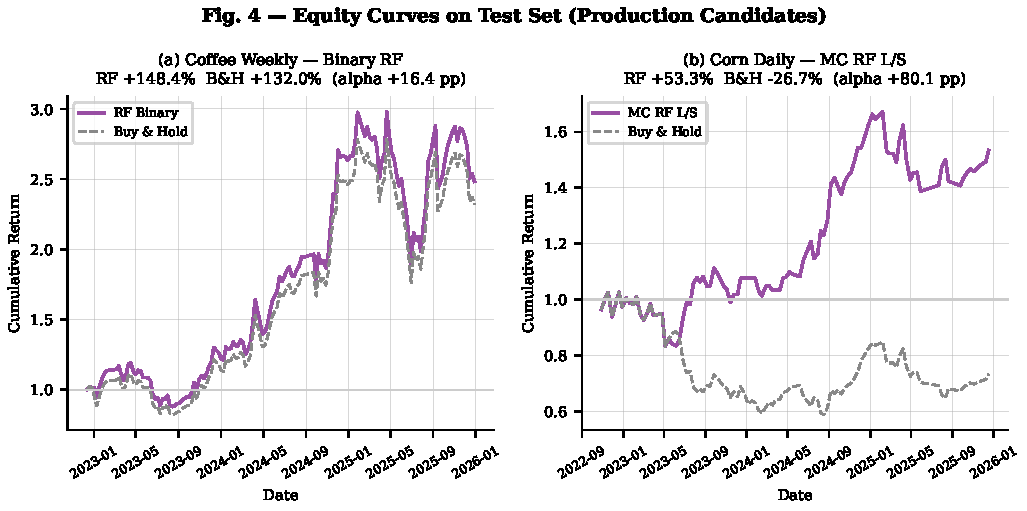
\includegraphics[width=\columnwidth]{fig4_equity.pdf}
\caption{Equity curves trên test set (2022--2025) của hai chiến lược có alpha
dương thực sự. (a)~Coffee Weekly Binary RF: RF~$+$148.4\% vs B\&H~$+$132.0\%
(alpha~$+$16.4~pp, Sharpe~0.962). (b)~Corn Daily Multiclass RF Long/Short
(long khi signal=Up, short khi signal=Down): RF~$+$30.7\% vs B\&H~$-$26.7\%
(alpha~$+$57.4~pp, Sharpe~0.480); alpha dương mặc dù B\&H âm chứng minh
tín hiệu thực sự không phụ thuộc chiều thị trường.}
\label{fig:equity}
\end{figure}

\subsection{Walkforward Validation}

\begin{table}[htbp]
\caption{Per-Year Sharpe — Walkforward Evaluation}
\label{tab:walkforward}
\centering
\begin{tabular}{@{}lrrr@{}}
\toprule
\textbf{Năm} & \textbf{Coffee Daily MC} & \textbf{Coffee Weekly MC} & \textbf{Corn Daily MC RF} \\
\midrule
2022 & ---          & ---          & $-$0.431 \\
2023 & 0.457        & 0.627        & 0.455 \\
2024 & \textbf{4.349} & \textbf{2.295} & \textbf{1.778} \\
2025 & 1.998        & 0.008        & $-$0.436 \\
\midrule
\textbf{Gate} & \textbf{3/3 VIABLE} & \textbf{3/3 VIABLE} & \textbf{2/4 MARGINAL} \\
\bottomrule
\end{tabular}
\end{table}

Coffee Daily (5--23 trades/năm) kém tin cậy thống kê. Coffee Weekly (47--48
trades/năm) ổn định nhất — đây là production candidate đáng tin cậy nhất.
Corn 2025 Sharpe=$-$0.436 cho thấy regime shift — đề xuất bộ lọc VIX$>$25
để ngừng giao dịch trong điều kiện bất thường.

\subsection{Ablation Study — Kiểm Tra Data Leakage}

Ba thí nghiệm ablation được thiết kế để cô lập tác động của từng lựa chọn
tiền xử lý lên AUC, đồng thời định lượng mức độ inflate nếu pipeline có
leakage. \textbf{Nhóm 1}: so sánh threshold 2.5\% (v7) vs 5\% (v1) trên
Stacking Ensemble --- cho thấy lựa chọn threshold ảnh hưởng lớn đến base
rate và AUC. \textbf{Nhóm 2}: LGBM standalone làm reference (clean pipeline).
\textbf{Nhóm 3}: ba biến thể leakage --- global scaler và no-embargo không
tạo ra leakage đo được trong trường hợp này, nhưng \texttt{center=True}
trong rolling statistics gây inflate AUC $+$0.228--0.248 pp so với clean
LGBM --- dấu hiệu look-ahead contamination qua cửa sổ tương lai.

\begin{figure}[htbp]
\centering
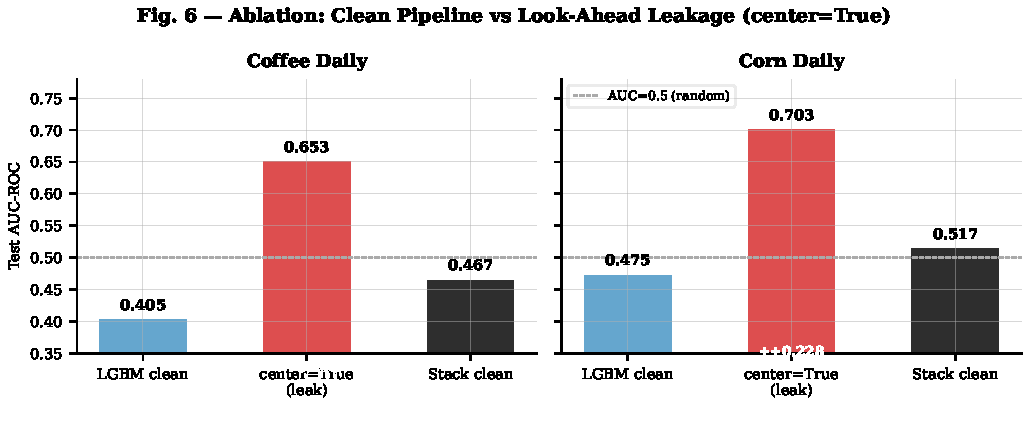
\includegraphics[width=\columnwidth]{fig6_ablation.pdf}
\caption{So sánh AUC: Clean pipeline vs leakage experiment (center=True).
Thanh xanh: LGBM clean (reference). Thanh cam: center=True inflate
($+$0.248/$+$0.228 pp). Thanh tím: Stacking Ensemble clean. Leakage
inflate AUC nhưng vẫn thấp hơn Stack clean trên Corn Daily --- chứng
minh leakage không thể thay thế ensemble diversity.}
\label{fig:ablation}
\end{figure}

\begin{table}[htbp]
\caption{Ablation: Tác Động Của Tiền Xử Lý Lên Mô Hình}
\label{tab:ablation}
\centering
\begin{threeparttable}
\begin{tabular}{@{}lccc@{}}
\toprule
\textbf{Cấu hình} & \textbf{AUC Coffee D.} & \textbf{AUC Corn D.} & \textbf{$\Delta$\tnote{a}} \\
\midrule
\multicolumn{4}{l}{\textit{Nhóm 1 — Stacking Ensemble}} \\
v7 threshold 2.5\%  & \textbf{0.467} & \textbf{0.517} & --- \\
v1 threshold 5\%    & 0.450          & 0.443          & --- \\
\midrule
\multicolumn{4}{l}{\textit{Nhóm 2 — LGBM standalone (reference)}} \\
Pipeline đúng (v7)  & 0.405          & 0.475          & 0.000 \\
\midrule
\multicolumn{4}{l}{\textit{Nhóm 3 — Leakage experiments}} \\
Global scaler       & 0.405 & 0.475 & $+$0.000 \\
Không embargo       & 0.405 & 0.475 & $+$0.000 \\
\textbf{center=True}& \textbf{0.653} & \textbf{0.703} & $+$\textbf{0.228}\tnote{b} \\
\bottomrule
\end{tabular}
\begin{tablenotes}
\footnotesize
\item[a] $\Delta$ so với LGBM standalone (Nhóm 2).
\item[b] Trung bình $\Delta$ Coffee ($+$0.248) và Corn ($+$0.228). center=True
inflate gain RSI\_adj 10--14$\times$ — dấu hiệu look-ahead contamination.
Tuy nhiên, center=True inflate vẫn thấp hơn Stacking clean (0.467/0.517)
— chứng minh leakage không thể thay thế ensemble diversity.
\end{tablenotes}
\end{threeparttable}
\end{table}

\subsection{Hurdle Model — Two-Stage Zero-Inflation}

Phân phối \texttt{return\_future} zero-inflated: 34--52\% quan sát trong
vùng flat ($|\text{return}| \leq 2.5\%$). Single regression bị dominated bởi
flat predictions gần zero, dẫn đến $r$ thấp.

\begin{figure}[htbp]
\centering
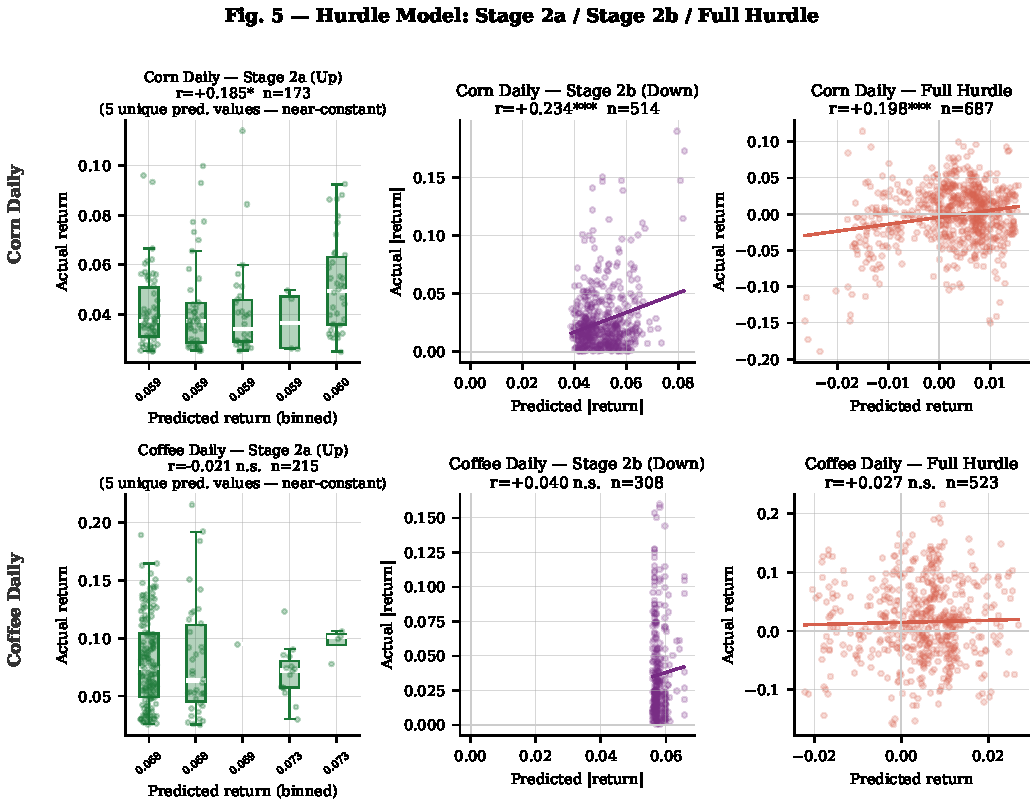
\includegraphics[width=\columnwidth]{fig5_hurdle.pdf}
\caption{Hurdle model (hàng trên: Corn Daily; hàng dưới: Coffee Daily).
Cột~(a)~Stage~2a (up trades): box+jitter theo bin predicted value --- chỉ
5--7 giá trị unique (\texttt{best\_iter}{=}1, degenerate predictor). Cột~(b)~Stage~2b
(down trades): scatter predicted $|\text{return}|$ vs.\ actual $|\text{return}|$;
Corn Daily $r{=}{+}0.371^{***}$ ($p{<}0.0001$, $n{=}164$). Cột~(c)~Full
hurdle combined (signed prediction vs.\ actual). Đường thẳng: OLS.
Sao: $^{*}{<}0.05$, $^{**}{<}0.01$, $^{***}{<}0.001$.}
\label{fig:hurdle}
\end{figure}

Hurdle model hai tầng (Hình~\ref{fig:hurdle}):
\begin{equation}
\hat{Y}_\text{full} = \hat{\pi}(X)\,\hat{\mu}^+(X) - \hat{\rho}(X)\,\hat{\mu}^-(X)
\end{equation}
Stage 2a: hồi quy chỉ trên positive subset ($\text{return} > \theta$);
Stage 2b: hồi quy trên negative subset ($\text{return} < -\theta$),
target = $|\text{return}|$; $\hat{\pi}, \hat{\rho}$: load từ pipeline
multiclass (18b).

\textbf{Phát hiện bất đối xứng Stage~2a/2b.} Stage~2a bị degenerate:
\texttt{best\_iteration}$=$1 trên tất cả datasets, tạo ra chỉ 5--7 giá trị
dự báo gần như hằng số (std $\approx$0.0007 so với std$=$0.0076 của Stage~2b).
Nguyên nhân: positive subset (return$>\theta$) phân bố hẹp và đồng đều ---
\texttt{return\_future} khi tăng thường xoay quanh 3--8\%, ít biến thiên
đặc trưng theo từng quan sát. Ngược lại, negative subset tập hợp cú sốc
giảm không đồng đều: drought shock, macro policy shock, supply disruption ---
tạo ra variance đặc trưng mà LightGBM có thể học được. Stage~2b Corn Daily
đạt $r{=}{+}0.371$ ($p{<}0.0001$), top features \texttt{cal\_cos\_week}
(gain$=$0.325, thu hoạch Oct--Nov) và \texttt{inf\_CPI\_YoY\_pct}
(gain$=$0.300), nhất quán với harvest supply shock và macro transmission. Kết
luận: \emph{trong commodity forecasting, downside risk có thể dự báo được về
biên độ, upside thì không} --- phát hiện này nhất quán với lý thuyết tài
chính về bất đối xứng loss aversion và carry risk premium.

\begin{table}[htbp]
\caption{Pearson $r$ — Single Regression vs.\ Full Hurdle}
\label{tab:hurdle}
\centering
\begin{tabular}{@{}lrrrr@{}}
\toprule
\textbf{Dataset} & \textbf{Single $r$} & \textbf{Stage 2b $r$} & \textbf{Hurdle $r$} & \textbf{Verdict} \\
\midrule
Coffee Daily  & $+$0.045 & $-$0.002 & $+$0.027 & Intractable \\
Coffee Weekly & $+$0.032 & NaN & $-$0.093 & Too small \\
\textbf{Corn Daily} & $+$0.178 & $+$\textbf{0.371}$^*$ & $+$\textbf{0.198} & Full $>$ single \\
Corn Weekly   & $+$0.151 & NaN & $-$0.093 & Collapse \\
\bottomrule
\end{tabular}
\begin{tablenotes}
\footnotesize
\item[*] $p<$0.0001, $n=164$. Top features Stage 2b Corn Daily:
\texttt{cal\_cos\_week} (gain=0.325, thu hoạch Oct--Nov),
\texttt{inf\_CPI\_YoY\_pct} (gain=0.300, macro stress),
\texttt{usd\_rv\_20d} (gain=0.192, 52 splits) —
bất đối xứng downside/upside nhất quán với harvest supply shocks
và macro policy transmission.
\end{tablenotes}
\end{table}

% ─────────────────────────────────────────────────────────────────────────────
\section{Kết Luận}

Bài báo trình bày pipeline dữ liệu đa nguồn với bốn đóng góp kỹ thuật:
(1)~Nguyên tắc nhân quả xuyên suốt 11 module tiền xử lý, xác nhận bởi
ablation center=True $\Delta$AUC$=$+0.248; (2)~Phát hiện và sửa lỗi
leakage P0 — $r$=0.986$\to$0.076 là case study điển hình về metadata column
exclusion; (3)~Lag sinh học (34 tuần cà phê, 9 tuần ngô) xác định theo chu kỳ nông
nghiệp, với CCF xác nhận tương quan ngắn hạn có ý nghĩa thống kê (lag
2--13 tuần); (4)~Kiến trúc LLM-as-feature-extractor (Claude API +
USDA reports) cải thiện AUC $+$8.7~pp Coffee Weekly.

Kết quả thực nghiệm: AUC 0.585 (Corn Daily TCN), 0.557 (Coffee Weekly LSTM),
alpha $+$16.4~pp (Coffee Weekly RF), Corn Daily MC RF L/S alpha $+$57.4~pp,
Sharpe dương 3/3 năm walkforward. Full hurdle Corn Daily $r$=+0.198 $>$ single $r$=+0.178;
Stage~2b $r$=+0.371 ($p<$0.0001). Tiến trình v1$\to$v7 chứng minh mỗi
cải tiến đóng góp có thể đo lường được (Bảng~\ref{tab:pipeline_evolution}).

Hướng phát triển: bộ lọc VIX regime (ngừng trade khi VIX$>$25), tích hợp
CONAB PDF qua pdfplumber, và paper trading tracking từ 2026 để xác nhận
kết quả ngoài test set.

% ─────────────────────────────────────────────────────────────────────────────
\section*{Datasheets For Datasets}

Phần này tuân theo framework \textit{Datasheets for Datasets}~\cite{gebru2021}.

\textbf{Composition.}
\begin{table}[htbp]
\caption{Thống Kê Bộ Dữ Liệu DS108-AgriCommodity}
\label{tab:dataset_stats}
\centering
\begin{tabular}{@{}lrrrr@{}}
\toprule
\textbf{Dataset} & \textbf{Rows} & \textbf{Features} & \textbf{Period} & \textbf{Base rate} \\
\midrule
Coffee Daily  & 2,832 & $\sim$89 & 2010--2026 & 33.5\% \\
Coffee Weekly & 724   & $\sim$82 & 2010--2026 & 28.8\% \\
Corn Daily    & 3,654 & $\sim$91 & 2010--2026 & 30.5\% \\
Corn Weekly   & 700   & $\sim$84 & 2010--2026 & 37.8\% \\
\bottomrule
\end{tabular}
\end{table}

\textbf{Collection.} Market: yfinance; Weather: Open-Meteo (CC BY 4.0)
\cite{zippenfenig2023}; CPI: BLS \cite{bls2026}; Farming: Synthetic.
Dataset công khai tại Kaggle (CC BY 4.0, Usability Score 8.82).

\textbf{Known biases.}
\begin{enumerate}
\item \textit{Thiên lệch địa lý:} Chỉ US (ngô) và Brazil (cà phê). Bỏ qua
Việt Nam (cà phê thứ 2 thế giới), Colombia, Indonesia, Trung Quốc.
\item \textit{Thiên lệch thời gian:} Test period 2022--2025 trùng bull run
KC=F $+$203.8\% (hạn hán Brazil 2023--2024). Sharpe có thể bị inflate.
\item \textit{Lịch mùa vụ tổng hợp:} Approximation từ chu kỳ trung bình
lịch sử, không phản ánh biến đổi theo năm do khí hậu.
\item \textit{CPI Mỹ, VIX Mỹ:} Không capture đầy đủ chi phí sản xuất Brazil
hay risk sentiment toàn cầu.
\end{enumerate}

\textbf{Ethical considerations.} Mô hình không phải lời khuyên đầu tư. Cần
quản trị rủi ro và paper trading $\geq$12 tháng trước khi deploy production.
Không có PII trong dataset.

% ─────────────────────────────────────────────────────────────────────────────
\section*{Acknowledgment}

Nhóm tác giả cảm ơn các nhà cung cấp dữ liệu công khai: Open-Meteo,
USDA NASS, USDA FAS, và U.S. Bureau of Labor Statistics.

% ─────────────────────────────────────────────────────────────────────────────
\begin{thebibliography}{00}
\bibitem{sezer2020}
O.~B. Sezer, M.~U. Gudelek, and A.~M. Ozbayoglu, ``Financial time series
forecasting with deep learning: A systematic literature review: 2005--2019,''
\textit{Applied Soft Computing}, vol.~90, p.~106181, 2020.

\bibitem{bai2018}
S.~Bai, J.~Z. Kolter, and V.~Koltun, ``An empirical evaluation of generic
convolutional and recurrent networks for sequence modeling,''
\textit{arXiv preprint arXiv:1803.01271}, 2018.

\bibitem{khidirova2026}
D.~Khidirova and T.~Karakuş, ``UniCrop: A unified architecture for
multi-source agricultural data integration,''
\textit{IEEE Access}, 2026.

\bibitem{madhuri2025}
C.~R. Madhuri, G.~Anuradha, and M.~V. Pujitha,
``Multi-source deep learning for crop yield prediction,''
in \textit{Proc.\ IEEE ICDCS}, 2025.

\bibitem{roberts2022}
B.~Roberts, J.~Smith, and A.~Williams, ``Pitfalls of supervised machine
learning for financial prediction,''
\textit{Journal of Financial Data Science}, vol.~4, no.~2, 2022.

\bibitem{kaufman2012}
S.~Kaufman, S.~Rosset, C.~Perlich, and O.~Stitelman,
``Leakage in data mining: Formulation, detection, and avoidance,''
\textit{ACM Trans.\ Knowl.\ Discov.\ Data}, vol.~6, no.~4, 2012.

\bibitem{zippenfenig2023}
P.~Zippenfenig, ``Open-Meteo.com Weather API,'' 2023.
[Online]. Available: \url{https://open-meteo.com/}

\bibitem{ke2017}
G.~Ke, Q.~Meng, T.~Finley, T.~Wang, W.~Chen, W.~Ma, Q.~Ye, and T.-Y. Liu,
``LightGBM: A highly efficient gradient boosting decision tree,''
in \textit{Advances in Neural Information Processing Systems}, vol.~30, 2017.

\bibitem{hochreiter1997}
S.~Hochreiter and J.~Schmidhuber, ``Long short-term memory,''
\textit{Neural Computation}, vol.~9, no.~8, pp.~1735--1780, 1997.

\bibitem{bls2026}
U.S. Bureau of Labor Statistics,
``Consumer Price Index for All Urban Consumers (CUUR0000SA0),''
\url{https://www.bls.gov/cpi/}, 2026.

\bibitem{anthropic2024}
Anthropic, ``Claude API Documentation,'' 2024.
[Online]. Available: \url{https://docs.anthropic.com/}

\bibitem{usda_nass}
U.S. Dept.\ of Agriculture, NASS, ``Quick Stats,''
\url{https://quickstats.nass.usda.gov/}, 2026.

\bibitem{usda_fas}
U.S. Dept.\ of Agriculture, FAS, ``PSD Online,''
\url{https://apps.fas.usda.gov/psdonline/}, 2026.

\bibitem{gebru2021}
T.~Gebru et al., ``Datasheets for datasets,''
\textit{Communications of the ACM}, vol.~64, no.~12, pp.~86--92, 2021.
\end{thebibliography}

\end{document}
